\documentclass[12pt,fleqn]{article}\usepackage{../../common}
\begin{document}
Değişimsel Calculus (Calculus of Variations) ve Euler-Lagrange Denklemi

İki nokta arasındaki en kısa mesafe hangisidir? Bu basit soru belki bizi
güldürmüştür çünkü cevabı çok iyi biliyoruz. Ama bu cevabı ispatlayabilir
miyiz? Birazdan bunu yapacağız. 

Ama birazdan işleyeceğimiz tekniklerin faydasını daha iyi belirtmek için
örneklere devam edelim; Dünya üzerindeki iki nokta arasındaki en kısa
yüzeysel mesafe sorulsa bunun bir çembersel bir yol olacağını biliriz. Ama
ya aynı soruyu mesela bir elipsoid ya da bir silindir ya da bir koni yüzeyi
için sorsak? Herhangi bir yüzey üzerinde iki nokta arası en kısa mesafe
soruları için değişimsel calculus kullanılabilir.

DC ile  minimum problemlerini çözmüş oluruz bir bakıma, aynen $f(x)$'in
minimum'unu bulmak için $f'(x) = 0$ yapıp işleme devam etmek gibi. Fakat DC
ile pek çok farklı fonksiyon arasından istediğimiz sonucu minimize eden
{\em özgün fonksiyonu} bulmaya uğraşıyoruz, tek bir fonksiyonun tek minimum
noktasını değil. Bu sebeple DC daha geniş problemler için kullanılabilir.

Örnek

Bir düzlem üzerindeki $x_1,y_2$ ile $x_2,y_2$ noktasını birleştiren en kısa
$y(x)$ eğrisini bulun.

Cevap

Doğru cevap tabii ki düz bir çizgi. Ama bunu bilmiyormuş gibi yapalım. 

Minimize etmek istediğimiz 

$$
I = \int _{x_1}^{x_2} \sqrt{ 1 + y'^2} \ud x
$$

Yani eğri uzunluğu. Üstteki formülün nereden geldiğini [5]'te
görebiliriz. İfadenin söylediği bulmak istediğimiz $y$ için öyle bir
$y = y(x)$ ``ekstremsel (extremal) değer'' bulmak ki $I$ en kısa
olsun. Şimdi bize aynı başlangıç, bitiş noktalarından geçen ama (hala
bilinmeyen) ekstremselden biraz farklılaşan tüm eğrileri cebirsel olarak
temsil etmenin bir yolu gerekli.

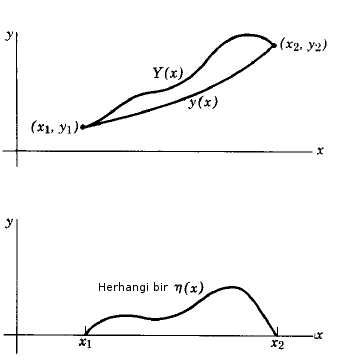
\includegraphics[width=15em]{phy_varcalc_01.png}

Bu farklı eğrileri şöyle temsil ediyoruz; diyelim ki $\eta(x)$ herhangi bir
fonksiyon olsun, bu fonksiyon $x_1$ ve $x_2$ noktalarında sıfır olmalı,
sürekli bir ikinci türevi var. Ama bunun haricinde $\eta$ herhangi bir şey
olabilir. Şimdi bir $Y(x)$ tanımlıyoruz,

$$
Y(x) = y(x) + \epsilon \eta(x) 
\mlabel{3}
$$

ki $\epsilon$ bir parametre. $\eta(x)$ herhangi bir şey olabileceği için
$Y(x)$ fonksiyonu da $(x_1,y_2),(x_2,y_2)$ noktalarindan geçen herhangi bir
eğri olabilir. Biz tüm bu eğriler içinden

$$
I = \int _{x_1}^{x_2} \sqrt{ 1 + Y'^2} \ud x 
\mlabel{2}
$$

formülünü minimal yapanı istiyoruz. Üstteki tanım sayesinde $I$ fonksiyonu
$\epsilon$'un fonksiyonu haline geldi. $\epsilon = 0$, ve $Y = y(x)$
değerleriyle ekstremsel değeri elde ediyoruz. Şimdi istediğimiz
$\epsilon=0$ iken $I(\epsilon)$'un minimum değerini almasını
sağlamak. Diğer bir deyişle 

$$
\epsilon = 0 \quad \textrm{için} \quad \frac{\ud I}{\ud \epsilon} = 0
$$

olmasını istiyoruz.

(2)'nin $\epsilon$'a göre türevini alalım, 

$$
\frac{\ud I}{\ud \epsilon} = \int _{x_1}^{x_2} 
\frac{1}{2} \frac{1}{\sqrt{1 + Y'^2}} 2Y' 
\left( \frac{\ud Y'}{\ud \epsilon} \right) 
\ud x
$$

Üstteki formüldeki $Y'$ değerini bulmak için (3)'un $x$'e göre türevi

$$
Y'(x) = y'(x) + \epsilon \eta'(x) 
\mlabel{4}
$$

Şimdi üsttekinin $\epsilon$'a göre türevi alınabilir,

$$
\frac{\ud Y'}{\ud \epsilon} = \eta'(x)
$$

Tüm bunları üç üstteki formüle geri koyarsak, 

$$
\left( \frac{\ud I}{\ud \epsilon} \right)_{\epsilon = 0} =
\int _{x_1}^{x_2} \frac{ y'(x)\eta'(x) }{\sqrt{1 + y'^2}} \ud x = 0
$$

Parcali entegrasyon uygulayabiliriz (cunku $\eta$ ve $y$'nin surekli ikinci
turevinin oldugunu farz etmistik zaten),

$$
u = y' / \sqrt{1 + y'^2}, \quad \ud v = \eta'(x) \ud x
$$

O zaman 

$$
\ud u = \frac{\ud}{\ud x} \left( \frac{y'}{\sqrt{1+y'^2}} \ud x \right),
\quad 
v = \eta(x)
$$

Yani

$$
\left( \frac{\ud I}{\ud \epsilon} \right)_{\epsilon = 0} =
\frac{y'}{\sqrt{1+y'^2}} \eta(x) \bigg\vert _{x_1}^{x_2} -
\int _{x_1}^{x_2} \eta(x) \frac{\ud}{\ud x} \left( \frac{y'}{\sqrt{1+y'^2}} \right)
\ud x
$$

Üstteki ifadede ilk terim sıfır olacaktır çünkü $\eta(x)$ üç noktalarında
sıfırdır. Geriye kalanların sıfır sonucunu vermesi için 

$$
\frac{\ud}{\ud x} \left( \frac{y'}{\sqrt{1+y'^2}} \right) = 0
$$

olmalıdır, yoksa, eğer bu ifade sıfır değilse herhangi bir $\eta(x)$
seçilebilirdi ve bu $\eta$ sıfır olma ihtimalini ortadan kaldırırdı. Nüansa
dikkat; diyoruz ki iki üstteki entegralin her zaman, her $\eta$ için sıfır
olmasının tek yolu üstteki ifadenin doğru (sıfır) olması.

Devam edersek üstteki formülü $x$'e göre entegre edersek, 

$$
\int \frac{\ud}{\ud x} \left( \frac{y'}{\sqrt{1+y'^2}} \right) \ud x = \int
0 \ud x 
$$

$$
 \left( \frac{y'}{\sqrt{1+y'^2}} \right) = \textrm{ sabit }
$$

Mantığa devam edelim, üstteki sabitlik $y'$ değerinin sabit olması
demektir. 

Demek ki $y$'nin eğimi sabit, eğimi sabit olan şey nedir? Bir düz çizgi! 

Oldukça iş yaptıktan sonra bir sonuca eriştik. Bu tür işlemleri her tür
problem için arka arkaya tekrarlayabilirdik, ama genel bir problem şablonu
için bu çözümü yapmak ve bir şablon sonuca erişmek çok daha rahattır,
böylece o şablon sonucu ardı ardına her yeni problemde kullanabiliriz, tek
gereken şablondaki değişkenlerin ne olduğuna bakmaktır, ve şablondan direk
sonucu alabiliriz.

Amac 

$$
I = \int _{x_1}^{x_2} F(x,y,y') \ud x
$$

entegralini durağan (stationary) yapacak $y$ fonksiyonunu bulmak, ki $F$
bize verilen bir fonksiyon. $I$'yi durağan yapan $y$'ye extremsel deniyor,
$I$ maksimum, minimum olsun farketmiyor. Metot biraz önce düz çizgi için
kullandığımız metot gibi, bir

$$
Y(x) = y(x) + \epsilon \eta(x)
$$

ile pek cok farkli egri dusunmek. Simdi 

$$
I = \int _{x_1}^{x_2} F(x,Y,Y') \ud x
$$

entegraline bakalım ve istediğimiz $\epsilon = 0$ iken
$ \ud / \ud \epsilon) ) I(\epsilon) = 0$ olması. $Y,Y'$ değerlerinin
$\epsilon$'un fonksiyonları olduğunu hatırlıyoruz, ve entegralin
$\epsilon$'a göre türevini alınca, 

$$
\frac{\ud I}{\ud \epsilon}  = 
\int _{x_1}^{x_2} \left(
\frac{\partial F}{\partial Y} \frac{\ud Y}{\ud \epsilon} + 
\frac{\partial F}{\partial Y'} \frac{\ud Y'}{\ud \epsilon} 
\right) \ud x
$$

(3) ve (4)'u üstteki formüle sokarsak, 

$$
\frac{\ud I}{\ud \epsilon}  = 
\int _{x_1}^{x_2}
\left[
\frac{\partial F}{\partial Y} \eta(x) + 
\frac{\partial F}{\partial Y'} \eta'(x) 
\right] \ud x
$$

$\epsilon = 0$ iken $ \ud / \ud \epsilon) ) I(\epsilon) = 0$ istiyoruz
demiştik, ve hatırlarsak $\epsilon = 0$ demek, $Y = y$ demekti. O zaman
üstteki 

$$
\left( \frac{\ud I}{\ud \epsilon} \right)_{\epsilon = 0} = 
\int _{x_1}^{x_2}
\left[
\frac{\partial F}{\partial y} \eta(x) + 
\frac{\partial F}{\partial y'} \eta'(x) 
\right] \ud x = 0
$$

olur. $y''$ değerinin sürekli olduğunu farzederek, üstteki ikinci terimi
aynen biraz önceki problemde olduğu gibi parçalı entegralle açmaya
uğraşacağız,

$$
\int _{x_1}^{x_2} \frac{\partial F}{\partial y'} \eta'(x) \ud x = 
\frac{\partial F}{\partial y'} \eta(x) \bigg\vert _{x_1}^{x_2} - 
\int _{x_1}^{x_2} \frac{\ud }{\ud x} \left( \frac{\partial F}{\partial y'}  \right)
\eta(x) \ud x
$$

Entegre edilmiş kısım sıfır çünkü önceki gibi $\eta(x)$ üç noktalarında
sıfır, o zaman 

$$
\left( \frac{\ud I}{\ud \epsilon} \right)_{\epsilon = 0} = 
\int _{x_1}^{x_2} \left[
\frac{\partial F}{\partial y} - 
\frac{\ud }{\ud x} \frac{\partial F}{\partial y'}
\right] \eta(x) \ud x = 0
$$

Yine biraz önceki gibi, $\eta$ herhangi bir fonksiyon olabileceği için,

$$
\frac{\partial F}{\partial y} - 
\frac{\ud }{\ud x} \frac{\partial F}{\partial y'} = 0
$$

olmalıdır. Üstteki formüle Euler denklemi ismi verilir. 

O zaman değişimsel Calculus'taki pek çok problem durağan olması istenen bir
entegral oluşturmak, $F$'in ne olduğunu ayarlamak, ve değişkenleri,
fonksiyonları üstteki Euler denklemine sokmak ve elde edilen (çok daha
basit) diferansiyel denklemi çözmektir.

Örnek

Başta gördüğümüz düzlem üzerindeki en kısa mesafe problemini yeni genel
metotumuz ile çözelim. Minimize etmek istediğimiz

$$
\int _{x_1}^{x_2} \sqrt{1 + y'^2} \ud x
$$

Yani $F =  \sqrt{1 + {y'}^2}$. O zaman,

$$
\frac{\partial F}{\partial y'} = \frac{y'}{\sqrt{1 + y'^2}}, \quad
\frac{\partial F}{\partial y} = 0
$$

Euler denklemine danışarak, $F,y,x$'leri yerine koyup,

$$
\frac{\ud}{\ud x} \left(
 \frac{y'}{\sqrt{1 + y'^2}}
\right) = 0
$$

elde ediyoruz. Bu biraz önce elde ettiğimiz sonuç ile aynı. 

Birden Fazla Değişken

Kendimizi tek bir bağımlı değişken $y$ ile sınırlamamıza gerek yok; temel
Calculus'tan hatırlarsak $z = z(x)$'te bir minimum nokta olması için
gerekli şart $\ud z / \ud x = 0$. İki değişkenli bir $z = z(x,y)$ için
gerekli iki şart var, $\partial z / \partial y = 0$ ve $\partial z
/ \partial x = 0$. 

Diyelim ki bize bir $F$ verildi ve bu $F$, $y$, $z$, $\ud y / \ud x$, $\ud z /
\ud x$, ve $x$'in bir fonksiyonu ve bulmak istediğimiz iki tane eğri,
$y=y(x)$ ve $z=z(x)$ öyle ki bu eğriler $I = \int F \ud x$ entegralini
durağan hale getiriyor. O zaman entegralin değeri hem $y(x)$ hem de
$z(x)$'e bağımlı olur ve tahmin edebileceğimiz gibi bu durumda iki tane
Euler denklemi gerekir, bir tane $y$ bir tane $z$ için, yani

$$
\frac{\ud}{\ud x} 
  \left( \frac{\partial F}{\partial y'} \right) -
  \frac{\partial F}{\partial y} = 0
$$

$$
\frac{\ud}{\ud x} 
  \left( \frac{\partial F}{\partial z'} \right) -
  \frac{\partial F}{\partial z} = 0
$$

Biraz önce tek değişkende gösterilen teknikleri kullanarak üsttekinin doğru
olduğunu ispatlayabiliriz.  


%%%%%%%%%%%%%%%%%%%%%%%%%%%%%%%%%%%%%%%%%%%%%%%%%%%%%%%%%%%%%%%%%%%%%

\newpage

Alternatif Anlatım

Değişimsel, Varyasyonel Calculus bir fonksiyon\textbf{el}in (dikkat
``fonksiyon'' değil) ekstrema (minimum / maksimum) ya da durağan
(stationary) olduğu noktaların bulunması için kullanılır.

Bir {\em fonksiyonel} bir veya daha fazla fonksiyonun
birleşimidir. Fonksiyonel girdi olarak bir fonksiyon alıp sonuç olarak
bir sayısal değer hesaplayan bir ikinci fonksiyondur aslında. Diğer
bir tanım fonksiyonelin belli fonksiyon ``tipleri'', ``sınıfları''
için bir sayısal değer ataması yaptığıdır.

Değimsel Calculus'un en temel, bilinen, standart problemi, sabit $x$
değerleri için alttaki fonksiyonelin (entegralin) durağan olduğu
$\phi(x)$ fonksiyonlarını bulmaktır. Yine dikkat: Bulmaya çalıştığımız
bir skalar $x$ değeri değil, bir veya daha fazla fonksiyondur.

$$ I(\phi)=\int_a^b F(x,\phi,\phi_x) \ud x $$

$\delta$ işareti varyasyon operatörüdür, ve diferansiyel operatörü
$d$'ye oldukça benzer. $\phi(x)$'nin varyasyon operatörü uygulanmış
hali olan $\delta \phi(x)$'in tanımı, sabit bir $x$ değeri için
herhangi (arbitrary), sonsuz ufaklıkta (infinitesimal) bir değişim
demektir. Doğal olarak $x$'in sabit olması $\delta x = 0$ anlamına
gelir (bu eşitliği birazdan formülümüzün açılımında basitleştirme
amacı ile kullanacağız). Fonksiyonelin durağanlığı da $\delta I = 0$
demektir.

Değişimsel Calculus ve Euler-Lagrange açılımının püf noktası altta
birazdan göreceğimiz cebirsel işlemlerle, $\delta \phi$'yi formülde
tek başına bırakarak bir anlamda durağanlık mantığının dışına
atmasıdır. Öyle bir $\phi(x)$ buluyoruz ki ondan $\delta$ sapmaları
var, ama biz oraya değil, formülün geri kalanına bakıyoruz, formülün o
tarafında üstünde sapmalar olmayan $\phi$ ile işlemler yapacağız, ve
optimal bir $\phi$ fonksiyonu bulacağız.

$I$ fonksiyoneli pek çok fizik, diğer tür problemlerde ortaya çıkan
bir formdur. Minimize edilmeye uğraşılan bir fonksiyonel var ise,
değişimsel calculus burada devreye girebilir, durağan nokta üzerinden
optimal bir $\phi(x)$ sonucunu verir.

Türetmeye başlayalım:

$\delta$ operasyonu diferansiyel ve entegral ortamlarında sırabağımsız
(commutative) özelliklere sahiptir, bu operasyonların içine ``nüfuz
edebilir''.  Mesela

$$ \delta \bigg( \int F \ud x \bigg) = \int (\delta F) \ud x $$

ve

$$ \delta \bigg( \frac{d\phi}{dx} \bigg) = \frac{d}{dx}(\delta \phi) $$

Üstte bahsettiğimiz fonksiyonelin varyasyonu o zaman

$$ \delta I = \delta \int_a^b F(x,\phi,\phi_x)\ud x = 0 $$

$$ = \int_a^b \delta F \ud x  $$

Şimdi $\delta F$'in açılımını gösterelim. Bu açılım tam diferansiyel (total
differential) açılımı ile tıpatıp aynı. 

$$ \delta I = \int_{a}^{b} \bigg(
\frac{\partial F}{\partial \phi}\delta\phi +
\frac{\partial F}{\partial \phi_x}\delta\phi_x +
\frac{\partial F}{\partial x}\delta x 
\bigg) \ud x
 $$

$\delta x = 0$ olduğunu bildiğimize göre bu terimi formülden
atabiliriz. Geri kalanlar:

$$ 
\delta F = 
\frac{\partial F}{\partial \phi}\delta\phi +
\frac{\partial F}{\partial \phi_x}\delta\phi_x  
$$

Bunları $\delta I$ formülünün içine koyarsak:

$$ 
\delta I  = \int_{a}^{b} (
\frac{\partial F}{\partial \phi}\delta\phi +
\frac{\partial F}{\partial \phi_x}\delta\phi_x 
) \ud x = 0
 $$

Entegraldeki ikinci terime bakalım: $\delta \phi$ formülünü $\delta
\phi_x$ formülü içinden ``çekip çıkartacağız''. Bunu niye yapıyoruz?
Çünkü $\delta \phi$'un herhangi (arbitrary) bir değere sahip
olabileceğinden hareketle ek bazı sonuçlara gelmeye çalışacağız, bu
da sadece $\delta \phi$'nin tek başına kalmasıyla mümkün olabilir.

$\delta$ operatörünün sırabağımsız olduğunu görmüştük. O zaman 

$$ 
\delta \phi_x = \delta \bigg( \frac{d\phi}{dx} \bigg) =
\frac{d}{dx}(\delta \phi)
 $$

$\delta \phi$'yi diferansiyel operatörünün içine attık. Şimdi parçalayarak
entegral alma (integration by parts) tekniğini kullanarak diferansiyel
operatöründen de kurtulacağız. Parçalayarak entegral alma bilindiği gibi 
şöyledir:

$$ \int_a^b u \cdot \ud v = u \cdot v - \int_a^b v \cdot \ud u $$

Eğer $\delta \phi$'in diferansiyelini $dv$'ye atarsak, o zaman parçalayarak
entegral alma tekniği $dv$'yi $v$ yaparken bize istediğimiz sonucu verecektir. O
zaman açmak istediğimiz entegrali hatırlayalım ve sırabağımsız işlemi uygulayalım:

$$
\int_{a}^{b} \frac{\partial F}{\partial \phi_x}\delta\phi_x \ud x =
\int_{a}^{b} \frac{\partial F}{\partial \phi_x} \frac{d}{\ud x}(\delta \phi) \ud x 
\mlabel{1}
$$

Parçalayarak entegral alma tekniği için parçaların ne olduğunu tanımlayalım:

$$ u = \frac{\partial F}{\partial \phi_x}  $$

$$ du  = d \bigg( \frac{\partial F}{\partial \phi_x} \bigg) $$

$$ dv  = \frac{d}{dx}(\delta \phi)dx = d(\delta \phi) $$

$$ v  = \delta \phi $$

O zaman (1)'ın açılımı şöyle olacaktır:

$$ 
\frac{\partial F}{\partial \phi_x} \delta \phi \bigg|_a^b - 
\int_a^b \delta \phi \cdot \ud \bigg( \frac{\partial F}{\partial \phi_x} \bigg)
 $$

Sağdaki terime $dx$'leri eklersek:

$$ 
\frac{\partial F}{\partial \phi_x} \delta \phi \bigg|_a^b - 
\int_a^b \delta \phi \cdot \frac{d}{\ud x} \bigg( \frac{\partial F}{\partial \phi_x} \bigg) \ud x
 $$

Görüldüğü gibi $\delta \phi$'in diferansiyelinden tamamen kurtulduk. Şimdi bu
sonucu $\delta I$ içindeki ikinci terim yerine koyalım:

$$ 
\delta I  = \int_{a}^{b} 
\bigg[ \frac{\partial F}{\partial \phi}\delta\phi -
\delta \phi \cdot \frac{d}{dx} \bigg( \frac{\partial F}{\partial \phi_x} \bigg)
\bigg] \ud x - \frac{\partial F}{\partial \phi_x} \delta \phi \bigg|_a^b 
$$

$\delta \phi$'ları dışarı çıkartalım:

$$ 
\delta I  = \int_{a}^{b} \bigg[
\frac{\partial F}{\partial \phi} -
\frac{d}{dx} \bigg( \frac{\partial F}{\partial \phi_x} \bigg)
\bigg] \delta\phi \ud x - \frac{\partial F}{\partial \phi_x} \delta \phi \bigg|_a^b 
$$

Bu sonuç üzerinden bazı ek mantık yürütmeye başlayabiliriz. Mesela $\delta \phi$
(belli sınırlar dahilinde olmak şartıyla) herhangi bir değere sahip olabileceği
için, o zaman $\delta I$'in sıfır olması demek, $\delta \phi$'in sıfır olması
garanti olmadığı için (herhangi bir değer dedik ya) $\delta \phi$'in içinde
olduğu çarpımda onun {\em haricindeki} değerlerin sıfır olmasını mecbur
kılacaktır. Bu demektir ki

$$ 
\bigg[
\frac{\partial F}{\partial \phi} -
\frac{d}{dx} \bigg( \frac{\partial F}{\partial \phi_x} \bigg)
\bigg] = 0
 $$

olmalıdır. Literatürde bu şarta Euler-Lagrange şartı ismi verilmiştir. Aynı
şekilde 

$$ \frac{\partial F}{\partial \phi_x} \delta \phi \bigg|_a^b = 0 $$

olmalıdır. Bu demektir ki ya $\delta \phi(a) = \delta \phi(b) = 0$ olacaktır, ki
bu şarta geometrik ya da kesinlikle gerekli sınır şartları (geometric or
essential boundary condition) denir, ya da

$$ \frac{\partial F(a)}{\partial \phi_x} = \frac{\partial F(b)}{\partial \phi_x} = 0 $$

olacaktır, bu şarta da doğal sınır şartı (natural boundary condition) ismi
verilir. 

Örnek

Şimdi örnek olarak iki nokta arasındaki en kısa eğrinin düz çizgi fonksiyonu
olması gerektiğini bulacağız. $F$ fonksiyonu nedir?

$$ F(x,y,y') = [1+(y')^2]^{1/2} $$

Bu fonksiyonun içinde $y$ olmadığına göre Euler-Lagrange'in $\phi$ (yani $y$)
içeren kısmın atabiliriz. Kalanlar:

$$ 
\bigg[
\frac{d}{dx} \bigg( \frac{\partial F}{\partial y'} \bigg)
\bigg] = 0
 $$

Parantez içindeki kısmi türevi hesaplayalım

$$
\frac{\partial F}{\partial y'}
= \frac{1}{2}[1+(y')^2]^{-1/2}\ 2y = \frac{y'}{[1+(y')^2]^{1/2}}
$$

Euler-Lagrange formülüne koyarak iki tarafın entegralini alalım ve $dx$'ten
kurtulalım:

$$ 
\int \bigg[
\frac{d}{dx} \bigg( \frac{y'}{[1+(y')^2]^{1/2}} \bigg)
\bigg] \ud x = c 
$$

$$ \frac{y'}{[1+(y')^2]^{1/2}}  = c $$

Sıfırın entegrali bir sabit sayı olacaktır, bu sabite $c$ ismini verdik. Şimdi
üstteki formülü $y'$ sol tarafta tek başına kalacak şekilde tekrar düzenleyelim:

$$ \frac{y'}{[1+(y')^2]^{1/2}}  = c  $$

$$ \frac{y'}{\sqrt{[1+(y')^2]}}  = c  $$

$$ \frac{y'^2}{1+(y')^2}  = c^2 $$

$$ \frac{1+(y')^2}{y'^2}  = \frac{1}{c^2} $$

$$ 1+\frac{1}{y'^2} = \frac{1}{c^2}  $$

$$ \frac{1}{y'^2} = \frac{1}{c^2} - 1 $$

$$ \frac{1}{y'^2} = \frac{1-c^2}{c^2}  $$

$$ y' = \sqrt{\frac{c^2}{1-c^2}} = a $$

Sağdaki sonuca bakarsak elimize geçen $c$'lerden oluşan bir işlem öbeğidir, ve
bu öbek te doğal olarak yine bir sabit sonucunu verir, bu sabite $a$ ismini
verdik. Devam edelim, $y'$, yani türevi bir sabit olan fonksiyon, $y(x)$ şuna
benzemez mi?

$$ y(x) = ax + b $$

ki sınır şartları $y(x)=x$ (0 ve 1 değerleri için). Bu formül bildiğimiz
gibi bir düz çizginin formülüdür! 

Demek ki Değişimsel Calculus kullanarak iki nokta arasındaki en kısa yolun düz
çizgi olacağını ispatlamış olduk.

Kaynaklar

[1] Everstine, G. C., {\em Numerical Solutions of Partial Differential Equations}

[2] Rao, S. S., {\em The Finite Element Method in Engineering}

[3] Thomas, {\em Thomas' Calculus, 11th Edition}

[4] Boas, {\em Mathematical Methods in the Physical Sciences, 3e}

[5] Bayramli, Çok Boyutlu Calculus, {\em 6. Ders}

\end{document}

